\section{Method}
\label{sec:method}
\begin{figure*}[t]
\centering
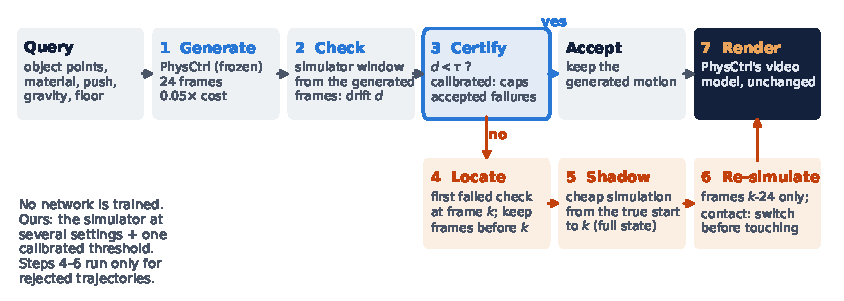
\includegraphics[width=\linewidth]{fig/method.pdf}
\caption{\textbf{Generate once, simulate only what fails.} A generated trajectory is checked by short simulator windows restarted from its own frames (\cref{sec:probes}) and certified by a calibrated threshold (\cref{sec:certificate}). A rejected trajectory keeps its certified prefix; only the rest is re-simulated, from a cheap shadow simulation of the true start (\cref{sec:repair}), and at contacts the shadow times the switch to a contact-resolving setting (\cref{sec:fidelity}).}
\label{fig:method}
\end{figure*}

\subsection{Problem and risk}
\label{sec:problem}
A query $q = (\mathbf{x}_0, \theta)$ consists of an object's initial particle positions $\mathbf{x}_0 \in \mathbb{R}^{N\times 3}$ and physical parameters $\theta$ (Young's modulus $E$, Poisson ratio $\nu$, drag forces, gravity, floor).
A generator $G$ (PhysCtrl's trajectory diffusion model~\cite{wang2025physctrl}) returns a trajectory $\hat{\mathbf{x}}_{1:T} = G(q)$ of $T = 24$ frames.
The reference simulator $S$ is the Material Point Method (MPM)~\cite{jiang2016material} solver that produced the generator's training data, run at its own setting; its rollout $\mathbf{x}_{1:T} = S(q)$ is the ground truth.
This is the motion the generator was trained to imitate, not real-world motion; we test its numerical convergence in \cref{sec:res-reference}.
% src: Phase 0 (replay error ~2e-6; same simulator for data and probes)
The error of a trajectory is the mean point distance $e(\hat{\mathbf{x}}) = \frac{1}{TN}\sum_{t,i} \lVert \hat{\mathbf{x}}_{t,i} - \mathbf{x}_{t,i} \rVert$, and a trajectory is \emph{bad} if $e > \varepsilon$.
We use $\varepsilon = 0.10$, about 5\% of the object size.
The \emph{risk} of a pipeline is the probability that its output is bad; its \emph{cost} is the compute it spends per query, relative to always running $S$.

\subsection{Sparse window probes}
\label{sec:probes}
A probe checks whether a short stretch of $\hat{\mathbf{x}}$ is consistent with physics.
At model frame $k$ we lift a simulator state $z_k$ from the generated frames: positions are read directly, velocities come from a three-point quadratic finite difference in time, the affine velocity field from a local least-squares fit over 12 neighbours, and the deformation gradient is set to the identity.
Lifting the deformation gradient from noisy generated positions made the simulator unstable even on ground-truth trajectories, while the identity never did.
% src: Phase 2 v1 NO-GO (F-lift blow-ups) vs Phase 2-v2 (lift_noF, 0 blow-ups)
We run a cheap simulator $S_c$ from $z_k$ for $m$ frames and measure the drift
\begin{equation}
  d_k = \tfrac{1}{N}\textstyle\sum_i \lVert S_c(z_k)_{k+m,i} - \hat{\mathbf{x}}_{k+m,i} \rVert .
\end{equation}
The defect needs no residual of the governing equations, only the simulator.
$S_c$ is the same MPM solver on a $64^3$ grid with a time step set by the CFL condition, $\Delta t = \min(8{\times}10^{-4}, 0.5\,\Delta x / c)$ for wave speed $c$; it keeps the signal of the reference setting at one eighth of the cost.
% src: Phase 2c verdict A' PASS
We use $m = 4$ frames.
For a single object, one window suffices: it starts at the strongest event in the generated motion (peak acceleration or floor proximity).
Two further windows spread over the remaining start frames rank errors no better (AUROC 0.958 vs.\ 0.955 on development data) at three times the probe cost.
% src: pilot E2 (exploratory, development data); placement spread_event chosen on Phase 2c by a pre-stated rule
For two-object scenes we keep all three windows: a generation that ignores a collision has no event at the collision, so the event window alone misses it.
% src: Phase 9 amendment before data (code check on seen 4o scenes: one window -> SF risk 0.095)
A window whose rollout blows up scores $d_k = +\infty$, an automatic reject.
% src: pre-registered Oct 10 (blow-up rule)
The certificate score is $s(\hat{\mathbf{x}}) = \max_k d_k$ over the placed windows.

\subsection{Object-level conformal certificate}
\label{sec:certificate}
We accept $\hat{\mathbf{x}}$ if $s(\hat{\mathbf{x}}) < \tau$ and calibrate $\tau$ on bad trajectories only.
Calibration queries come from objects that never appear at test time, several physical draws per object.
Because draws of one object are correlated, we calibrate at the object level: from each calibration object with at least one bad draw we pick one bad draw uniformly at random, and set $\tau$ to the $\lfloor \alpha (n+1) \rfloor$-th smallest of these $n$ scores.
For a new object exchangeable with the calibration objects, split conformal prediction then gives
\begin{equation}
  P\big(s(\hat{\mathbf{x}}) < \tau \,\big|\, e(\hat{\mathbf{x}}) > \varepsilon\big) \le \alpha ,
\end{equation}
so the risk of an accepted output is at most $\alpha\,P(e > \varepsilon)$.
With $\alpha = 0.10$ we obtain $\tau = 0.02614$ for the three-window score.
% src: Phase 4a extension (object-level), replicate 0; validity 0.084 <= 0.11 over 500 splits
The same calibration gives the one-window score a threshold of 0.0301; accepting a single window below the smaller $\tau$ accepts a subset of what that rule accepts, so the bound carries over.
% src: pilot E2 (variant a, threshold 0.03007); Phase 9 uses tau = 0.02614 for both
The guarantee holds in distribution. Under shift it is not guaranteed, and we test it empirically (\cref{sec:results}).

\subsection{Repairing only the uncertified suffix}
\label{sec:repair}
A rejected trajectory could be regenerated with its verified frames fixed.
We tried five such generative repairs, three training-free and two fine-tuned; the best improved the error by 1\% (\cref{sec:results}). A restart from generated states removes only 20\% of the error at its own frames, against 94\% from the true initial state, so verification does not supply correction; and optimising the generation against the defect lowered the defect while the true error doubled.
% src: Phase 4g-v2 diagnosis (20% vs 94%); Phase 4c (0.267 -> 0.511)
We therefore repair by simulation, and only where needed.

On rejection we walk a chain of windows: an anchor window from the true initial state, then windows starting at model frames $k \in \{3, 7, 11, 15, 19\}$, reusing windows the certificate already ran.
If the first failing window starts at frame $k$, we keep the generated frames up to $k$ and re-simulate the rest.
If the anchor fails, or no chain window fails, the whole trajectory is simulated with the reference setting.
The restart needs a full simulator state (positions, velocities, deformation gradients, affine velocities), which the generated frames cannot provide.
A \emph{shadow} supplies it: a cheap simulation from the true initial state up to frame $k$, whose full state starts the suffix.
% src: Phase 4h (restart from generated positions: risk 0.070) -> 4i V2 (shadow state: risk 0.017) -> 4k confirmation
The shadow is cheap and starts from the truth, so it carries the stress state that a restart from generated positions loses.

The suffix only has to meet the error target, not to reproduce the reference exactly.
We therefore run the shadow and the suffix at tuned settings of the same MPM solver:
the shadow at $\mathrm{M1}$ ($96^3$ grid, $\Delta t \le 8{\times}10^{-4}$) and the suffix at $\mathrm{M2}$ ($96^3$ grid, $\Delta t \le 4{\times}10^{-4}$), both capped at CFL number 0.5.
On development data this medium-fidelity suffix cut the cost of our pipeline by 25--55\% at similar risk.
% src: pilot 8a (exploratory, B2); Phase 9 confirmation uses M1 shadow + M2 suffix

\subsection{Event-aware fidelity at contact}
\label{sec:fidelity}
When two objects collide, the coarse grid cannot resolve the gap between them, so both the coarse check and the coarse shadow become unreliable near contact.
% src: Phase 4l diagnosis (dx 0.156 vs contact gap 0.16); 4l-ref H0 PASS at the reference setting
Instead of placing more windows at the contact, which did not help, we switch fidelity before it.
% src: Phase 4l H1-H3 FAIL
A coarse shadow from the true initial state records the distance between the two objects; at the first frame $k_{\mathrm{sh}}$ where they come within three coarse cells ($0.47$ units), a contact-resolving setting takes over from frame $\max(k_{\mathrm{sh}}-1, 1)$, restarted from the shadow's state.
This setting, $\mathrm{M3}$, uses the reference solver's $125^3$ grid with $\Delta t \le 2{\times}10^{-4}$; it was the cheapest setting within the error target on the development contact scenes.
% src: pilot 8a (M3 risk 0.004 on 4l contact scenes; M2 0.031); Phase 9 contact pipeline
If the shadow's objects start that close or never come that close, the scene is simulated with the reference setting.
Timing the switch from the generation instead, whose contact is itself wrong, narrowly missed its risk margin.
% src: Phase 4n N1 FAIL (0.034 vs 0.030); Phase 4o CONFIRMED

\subsection{Cost accounting}
\label{sec:cost}
All costs are A100 seconds per query: one generation costs 0.236\,s and one reference rollout 4.666\,s.
Probe windows are charged by a linear fit in simulator substeps, the shadow and the suffix by their substeps relative to a full reference rollout (the coarse shadow by its measured rate).
At 2{,}048 particles a substep costs almost the same on every grid we use (A100: 0.229\,ms at $64^3$, 0.233\,ms at $125^3$; H200: 0.29--0.32\,ms from $64^3$ to $125^3$), so charging simulator work by substeps treats all settings alike.
% src: p4d_fullsim coarse rate vs c_ref/20016 (A100); p9_full / p9c_full rollout_s per substep (H200), checked Oct 19
% src: Phase 1 timings; 4k cost model
